\documentclass[letterpaper,12pt]{article}

\usepackage[margin=1in]{geometry}
\usepackage{titling}
\usepackage{graphicx}

\setlength{\droptitle}{-0.75in}

\title{Fault Tolerance in Block-Level Caching}
\author{
  Jesus Ramos \\ \texttt{jramo028@fiu.edu} \and
  Douglas Otstott \\ \texttt{dotst001@fiu.edu}
}
\date{}

\begin{document}

\maketitle

\section*{Problem Statement}

Many companies are switching to warehouse scale computing to deal with
increasing computing demands due to the cost and efficiency of
warehouse architecture. Rather than trying to prevent failure, most
warehouse scale computing solutions accept failure and attempt to
integrate recovery as seamlessly as possible\cite{Placeholder}.
\\ \\*
Dependability and reliability are two important factors when dealing
with cloud and warehouse scale computing. Systems should be robust and
be able to recover from errors and failure effectively and quickly.
\\ \\*
Fault tolerance is still a major issue in cloud based systems that
employ caching. Currently in the event of an error or power failure
all data that was pending to be written back is lost along with
currently cached data. In some cases minor data loss is acceptable,
but in most cases even minor loss of data can result in larger
problems and error recovery can become very complex depending on the
type and quantity of data lost.

% end section Problem Statement

\section*{Problem Background}

\begin{center}
  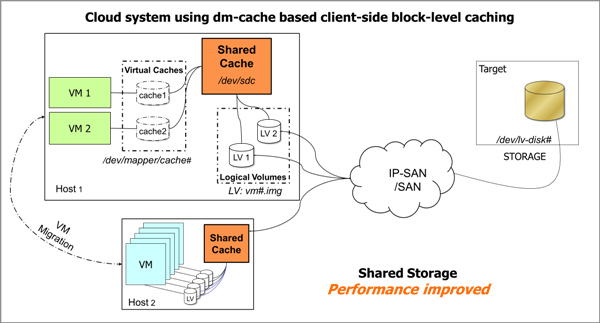
\includegraphics{../Images/NewerImage.png}
\end{center}
\noindent
Many large scale cloud based systems employ network storage due to the
physical limitations of local storage devices. Basically, each host
machine in the cloud is connected to a small number of machines which
are responsible for all persistent data management across the system.
These machines create what is known as a Storage Area Network (SAN).
SAN's are a common solution used by cloud service providers due to the
simplification of virtual machine migration and increased data
reliability. While this solves the storage size problem it also
increases the response latency and creates a bandwidth issue due to
the sheer volume of requests constantly sent to the storage devices.
\\ \\*
Local caches are employed by many systems as a means to bring in the
most frequently used data to more local storage devices to reduce
latency and alleviate pressure on the main storage system. DM-Cache is
an open-source block-level caching solution developed as a Linux
kernel module. DM-Cache allows host machines to store the most
recently used blocks in a designated storage device. Preliminary
testing on DM-Cache indicates a significant improvement in systems
where numerous hosts and virtual machines create a bottleneck in terms
of network storage bandwidth. However, local caching introduces a new
problem in terms of fault tolerance as locally modified blocks are lost
in the event of system failure.

% end section Problem Background

\section*{Proposed Solution}

The solution to the inherent fault intolerance of local caching is to move the
metadata from non-persisent memory to the persisent cahce device.  In this way, we
can reconstruct the state of the cache in the event of power loss or the host crashes 
to within some margin of error.  To minimize the performance overhead this policy would 
nessesitate, we also propose that recently used metadata should be cached in memory and 
changes to metadata should be written back to disk asynchronously.  This of course would
prevent very recent changes to metadata from being recovered if they had yet not been
commmited to disk.  However, we believe this is a fair trade off in terms of 
Fault Tolerance versus Performance.  

DM-Cache currently has two variantations in implmentation. One uses a hash table 
for a metadata structure and the other uses a radix tree. Currently, the plan is to
attempt implementation on both concurrently and focus on the either solution
in the interest of time. The radix tree implementation still has some bugs that still need to be 
addressed. Depending on the complexity of solving these issues, we may focus on the hash table
implementation in order to accomadate the projects time constrants. 

% add some stuff about how the metadata lets us make DM-Cache awesome
% also radix tree and hash table magic

% end section Proposed Solution

\section*{Project Timeline}

Feburary 26th - Begin Preliminary Testing (Radix Tree)
March 1st - Begin solution implementation (Radix/Hash)
April 5th - Debug solution (Hash Table)
April 10th - Begin Evaluation
April 15th - Conclude Evaulation
April 20th - Write a paper and present

% end section Project Timeline

\section*{Project Evaluation}

In this project we will evaluate the overhead introduced in DM-Cache
by persisting metadata to the disk.  The first round of testing will involve 
running I/O benchmarks with and without metadata persistance and compare the 
results to determine the performance decrease created by the extra overhead. 
The second test will evaluate the actual effectiveness of the data recovery mechanism.
The plan is to execute a standardize workload (such a kernel compilation) using a cache,
and we shall unplug the machine as the execution concludes.  We shall then measure the degree 
which data can be recovered in the metadata persistant cache vs the original dm-cache.

% more stuff about how this will help things do stuff faster

% end section Project Evaluation

\bibliography{proposal}
\bibliographystyle{plain}

\end{document}
